\documentclass[12pt, a4paper, oneside]{article} % Paper size, default font size and one-sided paper
%\usepackage[dcucite]{harvard}
%\usepackage{tikz}
%\usetikzlibrary{shapes, shadows, arrows}
%\usepackage{rotating}
\usepackage{amsmath}
%\usepackage{setspace}
%\usepackage{pdflscape}
%\usepackage[flushleft]{threeparttable}
%\usepackage{multirow}
\usepackage[comma, sort&compress]{natbib}% Use the natbib reference package - read up on this to edit the reference style; if you want text (e.g. Smith et al., 2012) for the in-text references (instead of numbers), remove 'numbers' 
\usepackage{graphicx}
\graphicspath{{./Figures/}} % Specifies the directory where pictures are stored
%\bibliographystyle{plainnat}

\bibliographystyle{agsm}
\usepackage[colorlinks = true, citecolor = blue, linkcolor = blue]{hyperref}
%\hypersetup{urlcolor=blue, colorlinks=true} % Colors hyperlinks in blue - change to black if annoying
\begin{document}
%\renewcommand[\harvardurl]{URL: \url}
\title{Carry trade and transission}
\author{Rob Hayward\footnote{University of Brighton Business School, Lewes Road, Brighton, BN2 4AT; Telephone 01273 642586.  rh49@brighton.ac.uk}} 
\date{\today}
\maketitle
\begin{abstract}
Hyman Minsky argued that financial instability would increase through an evolution that ran from stability to precarious instability, from one characterised by \emph{hedge financing} into successively more fragile regimes of \emph{speculative financing} and \emph{Ponzi financing}.  Though this process is not directly observable, there are financial market outcomes that are more likely to be prevalent in each of these regimes.  Analysis of \emph{carry trade} returns, the attempt to take advantage of deviations from \emph{uncovered interest partiy} (UIP), are used to identify the stages of increasing financial fragility.  Return characteristics change as financial instability develops so that the process can be modeled as a Markov chain where the states are unobserved but the outcome that are conditional on each state can be used to uncover the parameters of a Hiden Markov Model (HMM).   Identifying financial states can be used to aid understanding of financial system vulnerabilities and the triggers for the bursting of asset price bubbles. 

\end{abstract}

\section{Financial fragility}
The indiction from Federal Reserve Chairmn Ben Bernanke on 18th December 2013 that the central bank would cut back its pace of liquidity inject by gradully reducing its monthly bond purchase triggered a sharp sell-off in emerging bond and equity markets as well as their associated currencies.  This market reaction has brought attention back to relationship between US monetary policy and the flow of capital to emerging economies.  

One particular case for investing in emerging economies involves the \emph{carry trade}.  This is the attempt to take advantage of the breakdown in \emph{unovered interest parity}: the theory that interest rate differentials between currencies shoud be matched by an equal expectation that the low rate currency will appreciate against the higher rate until.  There is wide spread evidence that UIP does not hold on average.  However, it is debatble whether risk-free returns are possible.  There is a large body of research that suggests that these returns disappear with a more sophisticated assessment of risk that is being taken.  In particular, the small risk of a large loss, so-called \emph{crash risk} is either something that is to be avoided by most investors who are willing to pay to transfer this risk to other entities or is something that mis-perceived by myopic, over-coinfident economic agents suffereing behavioural biases.  

It is against this backdrop that a fuller appreciation of the build up of risk associated with carry-like trades is required. Hyman Minsky developed a model of endogenously increasing financial fragility.  The model suggests that a period of economic stability will provide the condidtions for a gradual transition of lending within the economy from one characterised as \emph{hedge} though that which is more \emph{speculative} and into something that can be desribed as {Ponzi}.  Under hedge financing the level of debt will not tend to extend beyond the ability to repay interest and principal; under specuative lending debt-to-equity ratios start to rise and the level of borrowing relative to income is elevated to a point where it becomes difficult to repay principal without asset price apprecation; under the Ponzi lending there is insufficient revenue to repay principal or interest and asset price appreciation or increased borrowing is necessary to mantain the debt. The Ponzi period tends to be sharp and explosive.

While this is a plausible description of rising financial fragility, it is often difficult to determine at what position the economy is at in the financial cycle.  While measuring debt-to-equity ratios and the scale of bank lending may provide some indication about the regime that is in place, this is imprecise and it is clear that financial services business evolve in ways that make loan counting in inadequate.\footnote{The recent financial crisis showed that innovations like \emph{Collateralised Debt Obligations (CDO)} can allow an increase in debt that does not directly in bank lending.}   Therefore, this paper proposes use an analysis returns that are achieved through a sample of potentil carry-trades to get a fuller understanding of the financial instbility process.  

The motivation for this research is to help to identify regimes and therefore help authorities determine the risk of financial crisis or crash. Use the FX market to get a broader understanding of some of the forces at work.

\section{Literature}
\subsection{Tapering and the Fed}
%This next paragraph does not work with the bibliograph.  Needs fixing. 
%There is a question about the extent to which the Fed-inspired sell-off in emerging markets is function of changes in liquidity and how much is a consequence of the change in risk-aversion. There are a number of studies that have looked at the effect of a change in Fed policy on capital flows to emerging markets.  For examp le, \citep{IMFLatam} argue that Fed tapering while not necessarily leading to capital outflow, could generate \emph{new risk premium shocks}.  These use a panel VAR method to assess the effect of US monetary policy since 1990 on capital flows to 38 emerging economies.  Similarly, \citep{NYFedtaper} assess how changes in global risk aversion affects carry trade activities.  They find that the initial signal from the US central bank in Fed Chairman Bernanke's May 22 2013 testimony to Congress coinciced with an increase in global risk aversion which affected global asset prices. They use the approach presented by \citep{MertensSVAR} to estimate the effect of policy changes by using a two-stage least squares appraoch to identify the SVAR model of asset price changes.  By identifying the performance of exchange rates without a change in risk aversion, they find that nearly half of the depreciation of a basket of 45 carry trade currencies with the largest one-month interest rate relative to a basket of the US dollar and other equally low rate currencies is explained by the increased risk aversion. Using a similar method they find that nearly all the decline in Emerging market equities is attributable to the increase in risk aversion. 

\subsection{Hidden Markov Models}
These models are used extensively in biometrics to analyse genome structure.  In particular, they are used to assess the underlying regime that is influencing the gene strcture. 

\href{http://a-little-book-of-r-for-bioinformatics.readthedocs.org/en/latest/src/chapter10.html}{Chapter 10 Biometric Text on HMM}
has an excellent overview of markov HMM and the R code necessary. One component of this that could be of interest is the assertion in on-line bimetrixs text that it is a problem to find the underlying state that produced the DNA outcome.  The equivalent of this for the crash model is to find the underlying Minsky state that produced the market activity. 

What is the probability of a particular pattern given a particular state. The three latent states are the periods of caution, build and crash.  These are unseen but may be identified by other variables (such as the level of international risk aversion (VIX) or the state of domestic political uncertainty (see that buy at Yale???)).  These periods can be compared to those uncovered by the crash model.  How well do these periods of political instbility compare to the hidden regimes tht are uncovered.  Alternatively, it may be possible to draw the states from the data and compare the information that is supplied by the data with that from what is known about political and economic developments at the time.  It is also possible to assess the probability that there will be a switch from one regime to another. 

There are two ways to try to identify the regimes: use external indicators such as the VIX index or other indications of domestic economic or political uncertaintly; use the internatl structure of the data to identify the periods through which the finncial system  is evolving. 

From Maatin's speech (can be deleted later).  In a \emph{mixture model}, each observation is assumed to be drawn from a number of distinct sub populations.  These can be called \emph{component distributions}.  The distribution from which the component is drawn is not immediately observable and is therefore represented as a \emph{latent state}. 

A mixture distribution is defined as 
\begin{equation}
p(Y_1 = y) = \sum_{i - 1}^N p(Y_t = y|S_t = i)P(S_t = i)
\end{equation}
where,
\begin{itemize}
\item $S_t \in {1, \dots, N}$ denotes the latent state or class of observation t
\item $P(S_t = i)$ denots the probability of the latent state t equals i 
\item $p(Y_t = y|S_t = i)$ denotes the density of observation of $Y_t$ conditional on latent state being $S_t = i$.
\end{itemize}

In the \emph{dependent mixture model} states are assumed to be statistically dependent.  This is consistent with the Minsky theory that the period of calm creates the conditions for the crash. The process underlying the state transitions is a \emph{homogenous first order Markov process}  (look this up for additional definition).  This process is completely defined by the initial state probabilities.  

\begin{equation*}
P(S_1 = 1), \dots P(S_1 = N)
\end{equation*}
and the state transition matrix, 

\begin{equation*}
\begin{pmatrix}
P(S_t = 1|S_{t-1}=1) & P(S_t = 2|S_{t-1}=1) & \dots & P(S_t = N|S_{t-1}=1)\\
P(S_t = 1|S_{t-1}=2) & P(S_t = 2|S_{t-1}=2) & \dots & P(S_t = N|S_{t-1}=2)\\
\vdots & \vdots & \ddots & \vdots \\
P(S_t = 1|S_{t-1}=N) & P(S_t = 2|S_{t-1}=N) & \dots & P(S_t = N|S_{t-1}=N)
\end{pmatrix}
\end{equation*}

The models are estimated using the Expectation-Maximisation (EM) or numerical optimisation (when parmeters are constrained).  The dependent mixture model is made up of three sub models:  
\begin{enumerate}
\item The prior model: $P(S_1|x, \theta_{prior})$
\item The transition model: $P(S_t|x, S_{t-1}, \theta_{trans})$
\item The response model: $P(Y_t| S_t, x, \theta_{resp})$
\end{enumerate}
 See Maarten's notes to see how these are implemented.  
 
\subsection{Agn Timmerman (2011)}
Looking at how abrupt changes in regime can lead to changes in the way that the system works.  The different regimes can be associated with different underlying distribution of returns.  This can allow the understanding of the non-liner and non--normal distribution within  normal or linear framework.  At the extreme, the regime switch model can incorporate a \emph{jump model} with one change, and can also be associated with time-varying parameter models that have a large number of regimes.

The broad framework for the method is to model a discrete state $s_t \in \{0,1,\dots k \}$
\begin{equation}
y_t = \mu_{s_t} + \phi_{s_t} y_{t-1} + \sigma_{s_t} \varepsilon_t, \quad \varepsilon_t \sim iid(0,1) 
\end{equation}

The process governing the underlying regime must also be defined. 

\begin{equation}
Pr(s_t = 0| s_{t-1} = 0) = p_{00} \quad \text{and} \quad Pr(s_t = 1| s_{t-1} = 1) = p_{11}
\end{equation}

More generally, the transition could be time-varying and could be dependent on the time spent in the regime.  See Durland and McCurdy (1994) for example of the probbilities  in the transition matrix being related to time. The longer the systemm has remained in the build phase, the greater the risk of crash.  Remember that the crash phase is a period when there is risk of a sharp reversal.  

See Diebold, Lee and Weinbch (1994) for examples where the transition probabilities depend on some other state variables.  For example, the interest rate spread.   Could the VIX index or other factors be used?  Vix index would indicate heightened international tension as one element that affects the probability of transforming from one state to the next.  An elevated VIX is an indication of the heightened international risk premium.  This may increase the probability that the regime switches from carry build to crash.  This is a theme that could be related to the bubble bursting so any information that improves the ability to identify bubbles bursting would be beneficial.  

The regimes are
\begin{itemize}
\item Hedge: cautious and risk averse
\item Speculative: More willing to take increased risk. 
\item Ponzi:  Risk-loving and explosive
\end{itemize}


In this case $p_{ij}(t) = \Phi(z_t)$, where $z_t$ is the conditioning informtion and $\Phi$ could be a logit or probit model.  There is logit in the switch from one to the other.  

\subsection{Hamilton, Palgrave}
From the Hamilton paper for the Plagrave dictionary, the transition matrix will determine the probility of switching from one regime to another.  If the transition has $b_{22} = 1$ this implies that the regime switch is permanent. More likely, it will be temporary. 
 
The use of the regime-switch allows the transition from one regime to another to be the result of something that is more than just a deterministic process. There are a number of ways that this model could be expanded.  Dueker has a model where the degrees of freedom from a Student-t distribution change with the regime.  

\subsection{Ghysels}
These notes from Ghysels.  There are two states of the world:  crisis and moderation.  If the system is in a crisis, it stays there with probability p; it switches to moderation with probability $1-p$.  If in moderation, the system stays there with a probability q and switches to crisis with probability $1-q$.  If the probabilities change over time, there is no longer a \emph{homogenous Markov Chain}. Ghysels has a seasonal dummy for the probabilities that represent the months or quarters.  

Can the probabilities change over time?  This may be the result of changes in the resilience of the financial system. 
\href{http://members.home.nl/jeroenvermunt/dias2010.pdf}{Mixture Hidden Markov Models} Hidden models help to calafify the regime under which securities trade. Model takes into account the unobserved hetrogeneity across time. This could could be extended to space (for different countries).  Is it possible to estimate a panel? 

Can the systemm be used to compare to fixed and floating exchange rates. 

\section{Methods}
\subsection{Data}
The data are a sample of CEE carry trades that have been compiled from raw exchange rate and interest rate data for the period from January 2000 to December 2012.  They show a range of possible carry trades that could have been conducted. 

The data are constructed with the function \emph{forp} in the \emph{Raw.R} file. This programme will create a sample of carry-trade profits from the inputs that will provide a funding currency from the set of US dollar, Euro, Swiss Franc and Japanese yen; an investment currency from the set of CEE countries provided; a time period of 1 month or 3 months.  Is there any need for any others funding curencies?  I don't think so!   It is possible to add other investment currencies.  There is ISK, TRY and NOK as reference.  It would be possible to have shorter time periods for the carry trade.   This would require the addition of the appropriate times series for LIBOR or deposit rates.  

The forumla for the carry can be taken from the doctorate. 

\subsection{Regime selection}
There are three states or regimes: the first is caution, the second is build and the third is caution. These three regimes or states loosely correspond to the three stages of financial instability: hedge finance, speculative finance and Ponzie finance. It is assumed that the Ponzie stage swiftly turns into a crash. 

Maybe put the R details in an appendix. 

The returns are modeled as a simple model of the level of returns and the standard deviation around this level.  it is assumed that there are three different regimes so the level and the standard deviation around this level is allowed to change with the regime.  

Three regimes are identfied with the 1-month investment in Polish zloty funded by US dollars.  These regimes are:  caution, carry-build and crash. 

\subsection{Wikipedia}
From wikipedia.  \href{http://en.wikipedia.org/wiki/Hidden_Markov_model}{Hidden Markov Models}.  The system is a Markov process.  There are unobserved, hidden states.  The Markov property A Markov chain satisfied the Markov property.  That means that it depends only on the current state.  It has no memory. \emph{Brownian motion}, for example, is a Markov process. In a Markov chain, the state is observed and the transition probabilities are the onl;y parameter.  In a HMM, each state has a probability distribution over the possible outcomes.  These can be called \emph{tokens}.  A series of \emph{tokens} can tell us someting about the states.   A hidden Markov model is a generalisation of the mixture model where hidden or latent variables are related through a Markov process. These latent variables comntrol the outcome token. A mixture model is a model with sub-populations where the observations do not allow identification of the sub populations.  A mixture model has a mixture distribution. A mixture distribution is a distribtion of a random variable that is derived from a number of random variales that are related to each other. If the variable is continuous, this is a mixture density.  The \emph{mixture components} are combined together to form the mixture distribution with certain \emph{mixture weights}.  Discrete are sometimes call \emph{compound distributions}.  There is a difference between adding together two normal distributons (where there will be a new normal with a new mean) and the mixture distibution (where there will be twin peaks).  

\href{http://members.home.nl/jeroenvermunt/dias2010.pdf}{Mixture Hidden Markov Models}  The observed response $y_{it}$ is the return of stock market $i$ at time $t$.  There are also two latent variables:  a time-constant discrete latent variable and a time-varying discrete latent variable.  The former is denoted by $w \in {1, \dots, S}$ captures unobserved hetoegeneity across markets; $z_t \in {1,2}$ is a two-state, time-varying latent variable. 

$f(y_{it}|z_t)$ is assumed to have a multivariate normal density function. This distribution is characterised by $\theta_k = (\mu_k, \sigma_k^2)$.  Excluding the states $w$, there are the initial state probabilities to be determined, the 2 transition probabilities and the conditional mean and conditional variance to be estimated.  Thsi is done by Maximum likelihood using the log-likelihood function $l(\varphi, y) = \sum_{i=1}^n log f(y_i; \varphi)$. This is a problem that can be solved with the \emph{Expectation-Maximization (EM) algorithm}.  Dempster, Laird and Rubin (1977).  The E step computes the joint conditional distribution of the latent variables given the data and the current provisional estimates of the model parameters. The M step ML methods are used to update the parameters using the estimated densities of the latent variables as weights. For hidden Markov models, as special variant of the EM algorithm is proposed (called \emph{the forward-backward} or \emph{Baum-Welch} alogorithm (Baum et al 1970).   

The markets are categorised as either \emph{bull} or \emph{bear} markets. This is consistent with the return volatility of markets.  About 25\% of the returns are in the bear markets. The evidence that the culster of markets that are closer to emerging markets are more liekly to be in a bear market than the devloped markets. In addition, it shows that there is persistence.  Once a market is in a particular regime (z) it is likely to stay there. Cluster 2 shows a lower propensity to move to a bear market from a bull market.  This is consistent with what is known about emerging markets.  The picture of the estimated posterior bull market regime is shown for emerging and deveped markets.  It shows that emerging markets are more likely to suffer bear markets.  

The second paper (on rating agencies - incuded in the "other" folder.  Uses the mixture model against the alternative of a pure Markov chain. In the pure Markov chain, the future depends only on the present.  However, with the mixture model, the future depends on the past.  This means that it is impant to know which of the latent sub-groups the firm is in as this will tell you more about the probability of default.  This knowledge will be based on the whole sample of ratings. There are A and Q processs.  What determines whether the rating evolves according to A or Q?  It appears to be partly the result of the industry.  The wholesale and retail trades are the most dynamic. There is clearly a hetrogeneity that is ignored by the standard Markov model of rating migration. 

Notes from the \href{http://www.comp.leeds.ac.uk/roger/HiddenMarkovModels/html_dev/main.html}{Leeds notes}.  The aim is to find patterns in time. This uses the examle of seaweed and traffic lights.  For the traffic lights, there is a state machine where the different states follow each other. Each state is dependent only on the previous state. This is a deterministic system. The weather is not deterministic.  There may be three states:  wet, cloudy and sunny. The Makov assumption says that the state depends only on the previous state. This is a simplification that makes the problem easier to solve.  Some information may be lost with the simplifcation. The Markov process moves from state to state, depending only on the previous n states.  This is called an \emph{order n model}, where n is the number of states affecting the choice of the next state. With the weather example there are 9 possible transformations $(M^2)$.  The probability of each transition is assigned  a probability called \emph{state transition probability}.  These are collected into a \emph{state transition matrix}. The probabilities do not vary with time.  This is a (unrealistic) assumption. To start the system, there is a \emph{vector of initial probabilities}.  This is the $\pi$ vector.  

The first order Markov process has three elements: 
\begin{enumerate}
\item states
\item $\pi$ vector
\item state tansmition matrix
\end{enumerate}
 Sometimes the Markov model is not sufficient to fully describe the process.  In the weather example, the weather may not be observable but seaweed is evident.  There is a probabilistic relationship between the seaweed and the weather.  More realistic is the identification of hidden states of the mouth through the sounds that can be identified.  The observables are related to the hidden states. It is assumed that the hidden states (the weather) are modelled by a simple first order Markov process.  The connections between the hidden states and the observable states represent the probability of generating a particular observed state given that the Markov process is in a particular state.  This is the \emph{confustion matrix} which gives the probabilites of observable states given a particular hidden state. 
 
The Hidden Markov Model (HMM) is a tripple $(\pi, A, B)$ where, 
\begin{enumerate}
\item $\pi$ Vector of initial state probabilities
\item $A = (a_{ij})$ the state transition matrix $Pr(x_{it}|x_{jt-1})$
\item $B = (b_{ij})$ the confusion matrix $Pr(y_i|x_j)$
\end{enumerate}

Once a system can be described as HMM, three problems can be solved. 
\begin{enumerate}
\item finding the probability of an observed sequence given a HMM (evaluation)
\item finding the sequence of hidden states that most probably generated the obsered sequence (decoding)
\item generating a HMM given a sequencde of observed observations (learning)
\end{enumerate}

\subsection{Evaluation}
There are a number of HMM with sets of $(\pi, A, B)$ tripples, which HMM geneated the given sequence?  For example, there may be 'summer model' and a 'winter model' and it may then be possible to determine the season from the seaweed sequence. The \emph{Forward algorithm} is used to calculate the probability of an observation sequence given a particular HMM and hence the most probable HMM.  In speech recognition, the HMM represent different words and the most likey HMM determines the word. 

\subsection{Decoding}
It is most usual to find the hidden states that generated the observed sequence.  Finding the hidden states is important because they are not directly observable.  A blind hermit may feel the seaweed but cannot see the weather. The \emph{Viterbi algorithm}.  This could also be used to determine the syntactic class of words (noune, verb etc) from the words themselves.  

\subsection{Learning}
This is the most difficult task.  Take a set of observations and fit the most probable HMM . The \emph{Forward-backward algorithm} is used when the A and B matrices are not directly (empirically) measurable.  

\section{Forward Algorithm}
With three states, three observations and the parameters of the model known, the aim is to find the most likely hidden sequence.  It would be possible to find each possible sequence and sum the probabilities.  





\section{Results}
Three regimes can be identified: number one, the cautious period; number two, the time when carry positions are being built; number three, the crash.  This works for PLNUSD, HUFEUR. 

The R files work as follows: prepare.R loads the data and creates the profits function; Raw(test).R will test data. 

\subsection{PLNUSD}
For the 1-month PLN-USD carry trade sample, a three stage HMM is fitted.  The parameters of the models are 

\begin{tabular}{l | l l}
State & Mean & SD \\
\hline
State 1 & 1.0109 & 0.0309\\
State 2 & 0.9317 & 0.0486\\
State 3 & 1.040982 & 0.0432\\
\end{tabular}

These figures have to extracted in some way 

 
\begin{figure}
\centering
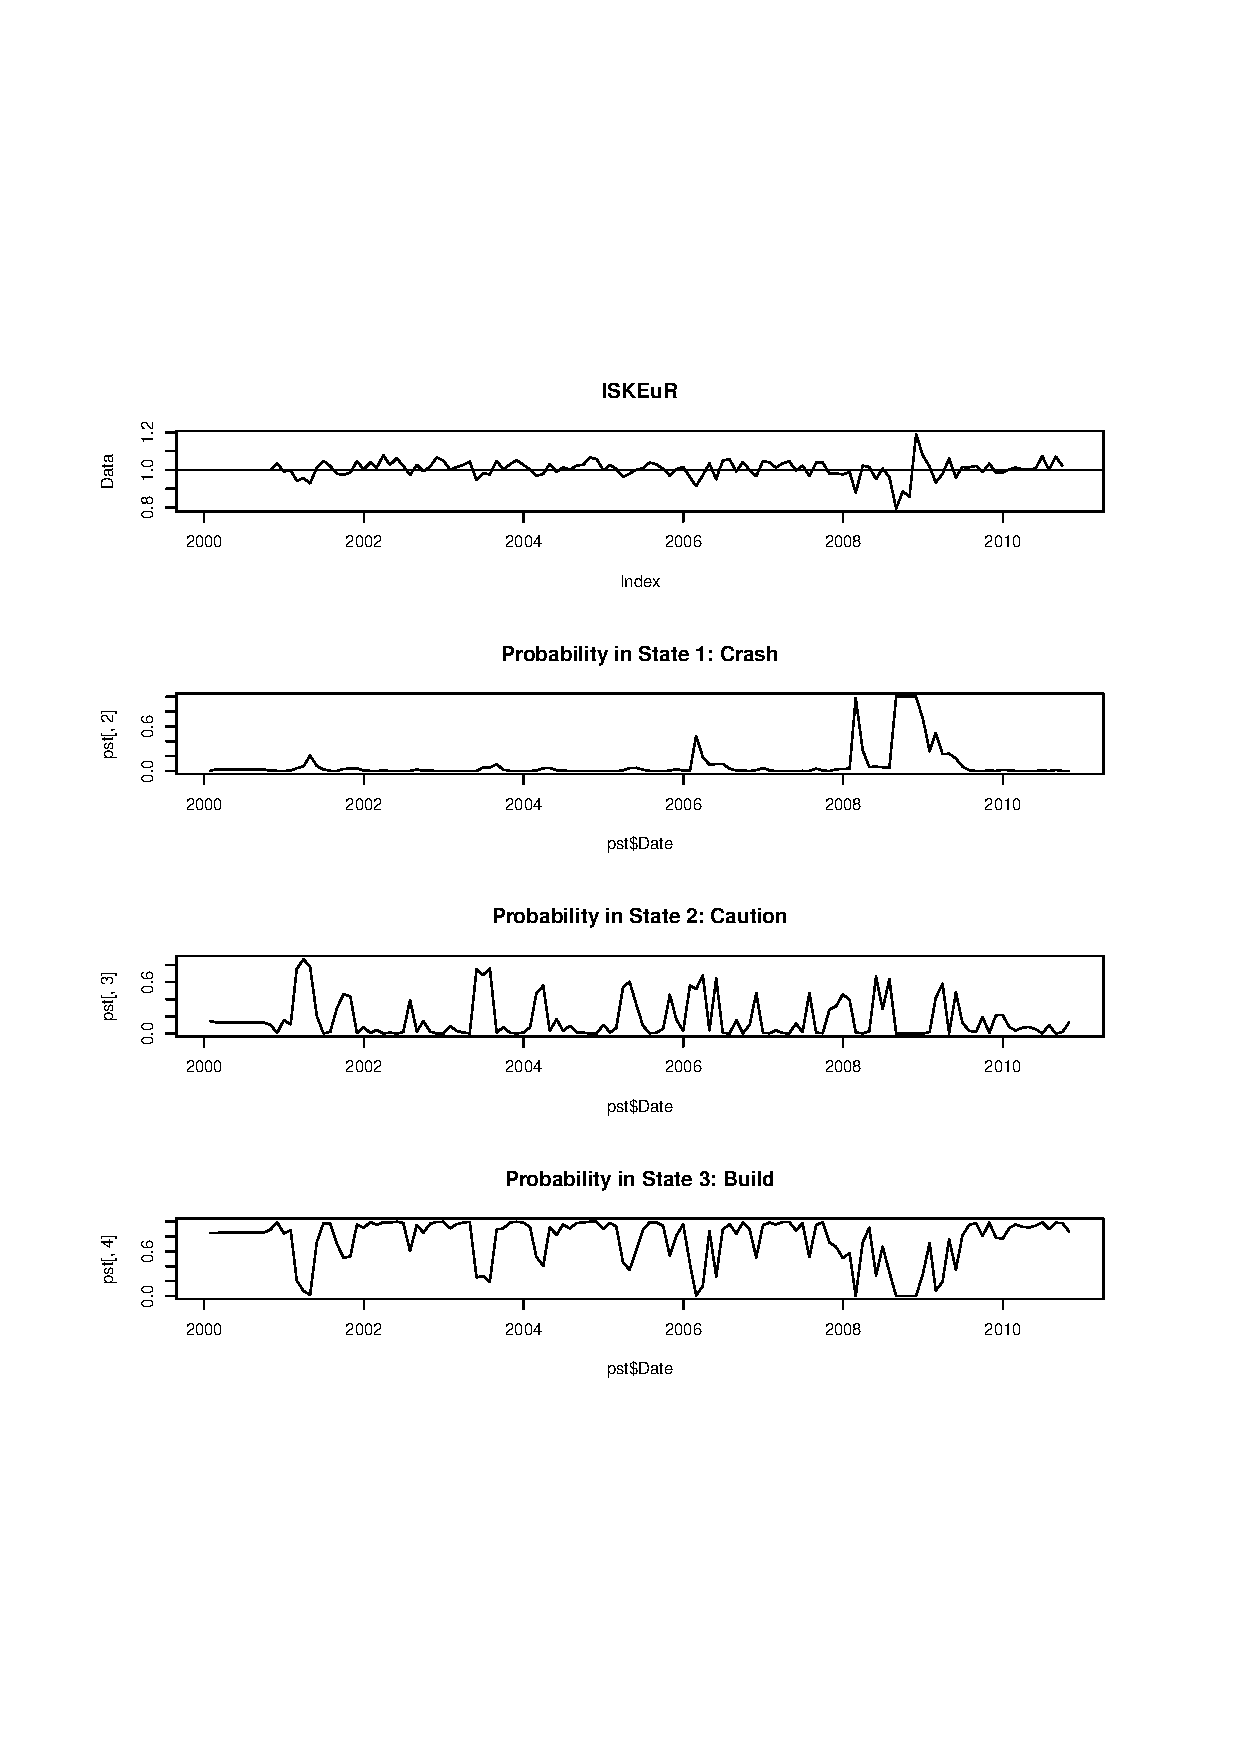
\includegraphics[scale = .80]{ISKEUR.pdf}
\end{figure}
% There are some issues with the creation of this figure.  It works in la tex stand alone.  

Need to update the regimes and the figures to get an overview.  Chose the countries to look at. 

The periods that are identified as those associated with the crash are July 2008 to January 2009 and April and May 2010.  

The Raw.R file works with the PLNUSD.  It gives the dates and the parameters of the model but it does not produce the pdf for the figures. Now this needs to be automated so that tables and figure can be produced automatically. Test on a couple of others. 

\section{Conclusions}
There are a number of ways that these methods can be used. 
\begin{itemize}
\item Looking at the changes in the probability that there is a crash and assessing the relationship between these changes and domestic and international events.  The doestic could be political opnion polls or central bank policy; the internatinal could be international risk or changes in Fed policy.  
\end{itemize}

\bibliography{myrefs}

\end{document}